%\addtocontents{toc}{\protect\newpage}
% {Youssouph Cissokho}
\newpage

\section{Anomalies et données de grande dimension}\label{Section:4}
%
La détection des valeurs aberrantes a été étudié dans le cadre d’un grand nombre de domaines d’application. De nombreuses données réelles sont de  grande (ou haute) dimension; dans certains scénarios, elles peuvent contenir des \textbf{centaines} ou des \textbf{milliers d'attributs}. \par Plusieurs méthodes classiques utilisent des concepts de proximité (distance) de détection d’anomalies (cf. Section 2) et ne sont valables que dans les cas où la taille d’échantillon $n$ est plus grande que la dimension $p$ ($n>p$).\newl La gestion des données de \textbf{haute dimension} ($n<p$) pr\'esente des difficult\'es particuli\`eres: les observations se retrouvent  \textbf{isolées} et \textbf{éparses}, et la notion de proximité ne parvient pas à conserver son pertinence. \par Ainsi, la notion de définition de valeurs aberrantes significatives est beaucoup plus complexe et moins évidente. Les cons\'equences de ce \textbf{fléau de la dimensionalité} sont d\'esastreuses pour les  méthodes conventionnelles de  détection des valeurs aberrantes, qui ne sont d\'esormais plus efficaces. \newl
Le reste de cette section est organisé comme suit: dans un premier temps, on pr\'esente une tentative de définition et certains des enjeux; on étudie ensuite les techniques de détection propre aux donn\'ees de haute dimension, en mettant l'accent sur las méthode des ensembles et des sous-espaces. On se réf\`ere principalement à \cite{A1,A8,A10,A14,Aurore}.

%
%
\subsection{D\'efinitions et défis}
%
%
Comme nous l'avons vu précédemment, une valeur aberrante est une observation qui s'écarte ou a des comportements différents des autres observations et dont nous  soup\-çon\-nons qu'elle a été générée par un autre mécanisme \cite{A1}. \newl
Les défis dans la détection des valeurs aberrantes ou anomalies en grande dimension réside dans le fait que,
\begin{itemize}[noitemsep]
\item la notion de distance ne parvient pas à conserver sa pertinence en vertu du fléau de la dimensionalité (c'est en ce sens qu'il est dit que ``le problème détection des valeurs aberrantes est comme trouver une aiguille dans une botte de foin'' \cite{A14});
\item chaque observation tend à devenir une valeur aberrante, et 
\item l'ensemble de données devient plus éparse avec une augmentation de la dimension.
\end{itemize}

\noindent Les auteurs de \cite{AYU} jugent qu'une approache valide pour les données de grande dimension doit tout au moins composer avec les aspects suivants \cite{Aurore}:
\begin{enumerate}[noitemsep]
\item la gestion efficace des problèmes liés à la rareté;
\item l'interprétabilité des r\'esultats;
\item la capacit\'e de comparer les mesures d'anomalie, et  
\item la prise en compte du comportement des données locales dans la détection des anomalies.
\end{enumerate}
%

%
\subsection{Méthodes de projection}
%
De nos jours, il est courant d'avoir de très grands ensembles de données connus sous l'acronyme HDLSS (``high dimension, low sample size''), c'est-\`a-dire \textbf{de haute dimension et avec une faible taille d'échantillon}, lesquelles peuvant contenir des centaines d'attributs (ou plus encore). \par Le fl\'eau de la dimensionalit\'e fait en sorte que les méthodes conventionnelles de  détection sont contre-indiqu\'ees. \newl 
Pour contrer ce problème, on peut utiliser la \textbf{r\'eduction de la dimensionalit\'e}, qui consiste à réduire la dimension de l'ensemble de donn\'ees tout en pr\'eservant l'essentiel de ses caractéristiques. Ces m\'ethodes de projection contiennent entre autres: 
\begin{itemize}[noitemsep]
\item l'analyse en composantes principales, 
\item l'analyse discriminante linéaire, 
\item la sélection des caractéristiques, etc. 
\end{itemize}
Nous discutons d'une de ces m\'ethods en d\'etail.%
\subsubsection*{Analyse en composantes principales}
%
L'\textbf{analyse en composantes principales} (ACP) cherche une représentation dans un sous-espace de dimension inférieure (tel une droite ou un plan) qui explique autant que possible la variation retrouv\'ee dans l'ensemble de donn\'ees original. 

Elle correspond à une  transformation linéaire orthogonale des données dans un nouveau système de coordonnées, telle que la plus grande variance résultant d’une projection scalaire des données se situe sur la première coordonnée (la \textbf{première composante principale}), la deuxième plus grande variance sur la seconde coordonnée, etc. 
\newl On rencontre l'ACP dans plusieurs contextes: 
\begin{itemize}[noitemsep]
    \item c'est une m\'ethode de réduction de la dimension utilis\'ee lors du  pré-traitement des donn\'ees;
    \item on s'en sert aussi pour visualiser les ensembles de donn\'ees, et, dans le sc\'enario qui nous int\'eresse, 
    \item on peut aussi s'en servir comme m\'ethode de detection des anomalies.
\end{itemize}
Étant donné une matrice des données $n\times p$, $\textbf{X}=[\textbf{X}_1,\cdots,\textbf{X}_p]$ à $n$ observations (nombre de lignes) et $p$ dimensions (nombre de colonnes) centrée et standardis\'ee, les \textbf{composantes principales} s'expriment par combinaisons linéaires: 
\begin{align*}
\textbf{Y}_i=\ell^{\!\top}_i\textbf{X}=\ell_{1,i}\textbf{X}_1+\cdots+\ell_{p,i}\textbf{X}_p;\quad i=1,\cdots,k,
\end{align*}
avec $k\leq p$, fournissant la plus grande variance sujet à la contrainte $\|\ell_i\|_2=1$. On en déduit alors que 
\begin{align*}
\operatorname{Var}\left(Y_{i}\right) &=\operatorname{Var}\left(\ell_{i}^{\!\top} \boldsymbol{X}\right)=\ell_{i}^{\!\top} \boldsymbol{\Sigma} \ell_{i} \,,\\ 
\operatorname{Cov}\left(Y_{i}, Y_{k}\right) &=\operatorname{Cov}\left(\ell_{i}^{\!\top} \boldsymbol{X}, \ell_{k}^{\!\top} \boldsymbol{X}\right)=\ell_{i}^{\!\top} \boldsymbol{\Sigma} \ell_{k}\, .
\end{align*}
Autrement dit, l'ACP cherche le vecteur $\ell_{1}$ qui  maximise la variance de $Y_1$, i.e. 
\begin{align*}
\mathbf{\ell}_{1}&=\underset{\|\mathbf{\ell_1}\|=1}{\arg \max }\left\{\ell^{\!\top}_1\mathbf{X}^{\!\top} \mathbf{X} \ell_1\right\},
\end{align*}
puis $\ell_2$ qui maximise la variance de $Y_2$ décorrélée de $\ell_1$, i.e.   
\begin{align*}
\mathbf{\ell}_{2}& =\underset{\|\mathbf{\ell_2}\|=1,\; \ell_{1}^{\!\top}\ell_{2} =0}{\arg \max }\left\{\ell^{\!\top}_2\mathbf{X}^{\!\top} \mathbf{X} \ell_2\right\}.
\end{align*}
De façon similaire, $\ell_k$ maximise la variance de $Y_k$ d\'ecor\'el\'ee de tout $\ell_i$, $i<k$, i.e. 
\begin{align}
\mathbf{\ell}_k=\underset{\substack{\|\ell_k\|=1,\\ \;\ell_{i}^{\!\top}\ell_k=0,\;\forall\;i<k}}{\arg \max} \left\{\ell^{\!\top}_k\mathbf{X}^{\!\top} \mathbf{X} \ell_k\right\}.\label{eq1}
\end{align}
On résoud \eqref{eq1} pour tout  $i<k$ \`a l'aide du  Lagrangien
\begin{align*}
L=\ell^{\!\top}_k\mathbf{X}^{\!\top} \mathbf{X} \ell_k-\lambda_k(\ell^{\!\top}_k\ell_k-1)-w\ell_{i}^{\!\top}\ell_k.
\end{align*}
On trouve les points critiques du Lagrangien en dérivant par rapport à chacune des composantes des vecteurs $\ell_k$, $\lambda_k$ et $w$, et en r\'esolvant par la mise \`a 0. En simplifiant, on obtient 
\begin{align*}
\mathbf{X}^{\!\top} \mathbf{X} \ell_k&=\lambda_k\ell_k\\
\ell^{\!\top}_k\ell_k&=1 \quad\text{et}\quad\ell^{\!\top}_k\ell_i=0,\quad\text{pour tout}\; i<k.
\end{align*}
Le vecteur $\ell_k$ recherché correspond au \textbf{vecteur propre associé à la} $k-$ième valeur propre en importance de la matrice de conception $\mathbf{X}^{\!\top} \mathbf{X}$. \newl
%\begin{lemma} Les $k$ ($k<p$ composantes principales donnant la plus grande variance maximale sont données par les $k$ vecteurs propres associés aux $k$ plus grandes valeurs propres de $\mathbf{X}^{\!\top} \mathbf{X}$.\end{lemma}
La \textbf{proportion de variance expliquée} se calcule en remarquant que
\begin{align*}
\sum_{i=1}^{p}\operatorname{Var}\left(Y_{i}\right) &=\sum_{i=1}^{p}\ell_{i}^{\!\top} \boldsymbol{\Sigma} \ell_{i}=\sum_{i=1}^{p}\lambda_i \,.
\end{align*}
Par conséquent, la proportion de la variance totale expliquée par la $i-$ème composante principale est 
\begin{align*}
0\leq \frac{\lambda_i}{\sum_{i=1}^{p}\lambda_i }\leq 1
\end{align*}
La qualité des résultats de l'ACP dépend fortement du nombres de composantes principales retenues, c'est-\`a-dire, de la dimension $k$ du sous-espace sur lequel on projette les donn\'ees. Il existe plusieurs méthodes qui traitent de ce problème -- nous n'en présentons que deux dans ce rapport.
\newl La part de variance totale expliquée par les $k$ premiers axes principaux est donnée par
\begin{align*}
p_k=\frac{\sum_{i=1}^{k} \lambda_i}{\sum_{i=1}^{p}\lambda_i}.
\end{align*}
On retient les $k$ composantes principales qui assurent que $p_k$  soit supérieure à une valeur prédéfinie (souvent comprise entre $80\%$ et $90\%$). \newl
La \textbf{méthode de l'éboulis} consiste à tracer la courbe des valeurs propres de la plus grande \`a la plus petite. Le principe consiste à repérer, s'il existe, un ``coude'' dans le graphe et de ne conserver que les valeurs propres (et donc les composantes principales correspondantes) jusqu'à ce coude.
\begin{Exemple}
L'ACP est appliquée sur les donn\'ees de mesures de l'expression génique chez $n=72$ patients atteints de leucémie, compos\'e de $p=7128$ gènes \cite{Hleukemia}. La courbe d'\'eboulis sugg\`ere de ne retenir qu'une seule  composante principale; la projection sur les 3 premi\`eres composantes principales est aussi disponible \`a la Figure \ref{fig0}.
\begin{figure*}[t]
    \centering
     \includegraphics[width=.58\textwidth]{ADOA/Images/screeleuk_\ldoc.png}
    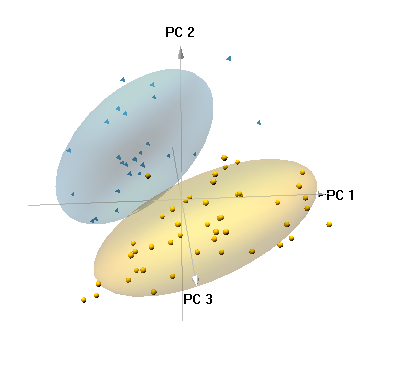
\includegraphics[width=.4\textwidth]{ADOA/Images/3dpcleuk.PNG}
    \caption{Courbe d'éboulis (\`a gauche); projection des données sur les 3 premi\`eres composantes principales (\`a droite).}\hrule
    \label{fig0}
\end{figure*}
\begin{lstlisting}
leukemia.big <- read.csv("http://web.stanford.edu/~hastie/ CASI_files/DATA/leukemia_big.csv")
leukemia.big <- t(leukemia.big)
leukemia.big.scaled <- scale(leukemia.big)
pca.leukemia <- prcomp(leukemia.big.scaled)
plot(pca.leukemia)
pca.leukemia.s <- summary(pca.leukemia) 
plot(pca.leukemia.s$importance[3,])
\end{lstlisting}
\end{Exemple}
\noindent Il y a diff\'erentes  m\'ethodes de r\'eduction de la dimensionalit\'e associ\'ees \`a l'ACP, telle que la d\'ecomposition par les valeurs singuli\`eres ou l'ACP du noyau; on retrouvera plus de d\'etails \`a ce sujet dans \cite{BLMMP}.
\newl Quel est le rapport avec la d\'etection des valeurs aberrantes? En g\'en\'eral, on peut s'arranger pour que la dimension du sous-espace sur lequel on projette soit de faible dimension -- c'est sur cet ensemble \`a dimension r\'eduite que l'on applique les m\'ethodes de d\'etection traditionnelles. Il va de soit que les r\'esultats seront affect\'es par la perte d'information qu'entra\^ine n\'ec\'essairement une telle projection, surtout si la présence ou l'absence d'anomalies n'est pas align\'ee avec les composantes principales de l'ensemble des donn\'ees. 

\subsubsection*{DOBIN}
Il y a un probl\`eme avec cette approche pour la d\'etection des anomalies: le type d'observation (normale ou aberrante) n'entre pas en jeu dans la construction de la base $\{\text{CP}_1,\ldots,\text{CP}_k\}$ sur laquelle l'ACP repose -- il n'y a pas n\'ec\'essairement de lien entre les directions de haute variance et la pr\'esence (ou l'absence) d'observations anormales. 
\newl 
L'algorithme DOBIN trouve une base qui est plus propice \`a la d\'etection des anomalies. L'id\'ee principale qui sous-tend DOBIN est de passer \`a la recherche de voisins imm\'ediats qui sont en fait \'eloign\'es les uns des autres: 
\begin{enumerate}[noitemsep] 
\item On commence par construire  un espace $\mathbf{Y}=\{\mathbf{y}_{\ell}\}$  qui contient $M\ll n(n+1)/2$  vecteurs de la forme $$\mathbf{y}_{\ell}=(\mathbf{x}_i -\mathbf{x}_j)\odot (\mathbf{x}_i -\mathbf{x}_j), $$ o\`u $\odot$ repr\'esente le produit d'Hadamard (multiplication \'el\'ement par \'el\'ement) et dont la magnitude en norme 1 $$\|\mathbf{y}_{\ell}\|_1=(x_{1,1}-x_{2,1})^2+\cdots +(x_{1,p}-x_{2,p})^2 $$ est le carr\'e de la distance euclidienne entre $\mathbf{x}_i,\mathbf{x}_j \in\mathbf{X}$ (le choix des $M$ paires d'observations se fait selon une proc\'edure assez complexe qui ne consid\`ere que $\mathbf{x}_i$ et $\mathbf{x}_j$ s'ils sont des $k-$voisins imm\'ediats, pour $k\in\{k_1,\ldots, k_2\}$); l'espace $\mathbf{Y}$ contient donc des points pour lesquels $\|\mathbf{y}_{\ell}\|_1$ est relativement \'elev\'ee, c'est-\`a-dire que les observations $\mathbf{x}_i$ et $\mathbf{x}_j$ sont relativement \'eloign\'ees m\^eme si ce sont des $k-$voisins imm\'ediats;
\item on construit ensuite une base $\{\eta_1,\ldots,\eta_p\}\subset \mathbb{R}^p$ o\`u chaque $\eta_i$ est un vecteur unit\'e obtenu par combinaison lin\'eaire particuli\`re d'\'el\'ements de $\mathbf{Y}$, en utilisant un proc\'ed\'e de type Gram-Schmidt: 
\begin{align*}
\mathbf{y}_{\ell_0}&=\mathbf{y}_{\ell},\quad \ell=1,\ldots, M \\ 
%\eta_1&=\frac{\sum_{\ell=1}^M\mathbf{y}_{\ell}}{\left\|\sum_{\ell=1}^M\mathbf{y}_{\ell}\right\|_2} \\
%\mathbf{y}_{\ell_1}&=\mathbf{y}_{\ell}-\langle\eta_1 \mid \mathbf{y}_{\ell}\rangle,\quad \ell=1,\ldots, M \\ 
%\eta_2&=\frac{\sum_{\ell=1}^M\mathbf{y}_{\ell_1}}{\left\|\sum_{\ell=1}^M\mathbf{y}_{\ell_1}\right\|_2} \\ 
\mathbf{y}_{\ell_{b-1}}&=\mathbf{y}_{\ell_{b-2}}-\langle\eta_{b-1} \mid \mathbf{y}_{\ell_{b-2}}\rangle,\quad \ell=1,\ldots, M \\ 
\eta_b&=\frac{\sum_{\ell=1}^M\mathbf{y}_{\ell_{b-1}}}{\left\|\sum_{\ell=1}^M\mathbf{y}_{\ell_{p-1}}\right\|_2},
\end{align*} pour $b=1,\ldots,p$,
\item et on transforme l'ensemble de donn\'ees original  $\mathbf{X}$ selon $\hat{\mathbf{X}}=\mathcal{T}(\mathbf{X})\Theta,$ o\`u $\mathcal{T}(\mathbf{X})$ normalise chaque attribut de $\mathbf{X}$ selon un syst\`eme appropri\'e au probl\`eme (Min-Max ou M\'ediane-\'Ecart interquartile, par exemple) et $$\Theta=[\eta_1\mid\cdots\mid \eta_p]$$ est une matrice unitaire de dimension $p\times p$.  
\end{enumerate}
C'est sur cet ensemble transform\'e (qui joue un r\^ole analogue \`a la projection de $\mathbf{X}$ dans l'ACP) que l'on applique les algorithmes de d\'etection des donn\'ees.\newl 
Les d\'etails de l'algorithme ne sont pas \'evidents et il y a plusieurs complications d'ordre technique; les lecteurs int\'eress\'es sont invit\'es \`a consulter \cite{A6} (l'algorithme est impl\'ement\'e dans le logiciel R \`a l'aide du module \textit{dobin}). 
%
\subsection{Méthodes ensemblistes}
%
%
Dans les sections précédentes, nous avons décrit divers algorithmes de détection d’anomalies dont les performances relatives varient avec le type de données considérées. Il est en g\'en\'eral   impossible de trouver un algorithme qui surpasse tous les autres. \par En effet, un algorithme de détection d'anomalie particulier peut être bien adapté à un ensemble de données et réussir à bien détecter des observations anormales ou aberrantes, mais peut ne pas fonctionner avec d’autres ensembles de données dont les caractéristiques ne concordent pas avec le premier ensemble de données. \par L'impact d'une telle inadéquation  entre algorithmes peut être atténué en utilisant la \textbf{ méthode des ensembles} où les résultats de plusieurs algorithmes sont considérés avant de prendre une décision finale. Cette approche fournit souvent les meilleurs résultats et améliore au passage les performances des algorithmes de d\'etection de base \cite{A10}. 
\newl Nous consid\'erons deux types de méthodes des ensembles: les \textbf{ensembles séquentiels} et les \textbf{ensembles indépendants}, 
\subsection*{Ensembles séquentiels}
Dans les ensembles séquentiels, un algorithme donné ou un ensemble d'algorithmes sont appliqués de manière séquentielle, de sorte \`a ce que les applications futures des algorithmes
réutilisent les résultats obtenus précédemment, et ainsi de suite. \`A chaque \'etape, le poids accord\'e \`a chaque observation est modifi\'e par les r\'esultats pr\'ec\'edents, \`a l'aide d'une m\'ethode de ``boosting'' (AdaBoost ou XGBoost, par exemple \cite{LB}). \newl Le résultat final prend soit la forme d'une combinaison pondérée de tous les résultats, ou le résultat final de la dernière application du dernier algorithme (consulter Algorithme~\ref{algSeq}). 

\begin{algorithm}
\SetAlgorithmName{Algorithme}{}
\SetAlgoLined
\textbf{Entr\'ees:} données $D$, algorithmes de base $A_1,\ldots,A_r$ 

$j=1$\;
\While{la condition d'arrêt n'est pas remplie}{
	Prendre un algorithme $A_j$ en se fondant sur les résultats des exécutions précédentes\;
	Créer un nouvel ensemble de donn\'ees $D_j$ \`a partir de $D$ en modifiant les poids de chaque observation en fonction des résultats des exécutions précédentes\;
	Appliquer $A_j$ à $D_j$\;
	$j=j+1$\;
}
\textbf{Sortie:} valeurs aberrantes obtenues en combinant les résultats des exécutions précédentes 
\caption{EnsembleS\'equentiel}\label{algSeq}
\end{algorithm}%\newl
\subsection*{Ensembles ind\'ependants}
Dans les ensembles ind\'ependants, on applique soit des algorithmes diff\'erents, soit  différentes instanciations
du même algorithme \`a l'ensemble de donn\'ees dans son entieret\'e (ou en partie, \`a l'aide de r\'e-\'echantillonage). \par Les choix effectu\'es au niveau des  données
et des algorithmes sont indépendants des résultats obtenus lors des ex\'ecutions pr\'ec\'edentes (au contraire des ensembles s\'equentiels). Les résultats sont ensuite combinées afin d'obtenir des valeurs aberrantes plus robustes (consulter l'Algorithme~\ref{algInd}).

\begin{algorithm}[t]
\SetAlgorithmName{Algorithme}{}
\SetAlgoLined
\textbf{Entr\'ees:} données $D$, algorithmes de base $A_1,\ldots,A_r$ 

$j=1$\;
\While{la condition d'arrêt n'est pas remplie}{
    Prendre un algorithme $A_j$\;
	Créer un nouvel ensemble de donn\'ees $D_j$ \`a partir de $D$, ind\'ependamment des résultats des exécutions précédentes\;
	Appliquer $A_j$ à $D_j$\;
	$j=j+1$\;
}
\textbf{Sortie:} valeurs aberrantes obtenues en combinant les résultats des exécutions précédentes 
\caption{EnsembleInd\'ependant}\label{algInd}
\end{algorithm}
\ \\
\noindent Chaque algorithme donne un score d'anomalie (ou une classification anormale/r\'eguli\`ere) \`a chaque observation de $D$; les observations qui reçoivent des résultats plus élevés sont considérés comme plus anormaux. On combine ensuite les résultats afin d'obtenir une classification des valeurs aberrantes ou anomalies plus robuste. Plusieurs techniques sont utilisées en pratique: \begin{itemize}[noitemsep]
\item le \textbf{vote à la majorité}, 
\item la \textbf{moyenne}, 
\item la m\'ethode du \textbf{rang minimal}, etc. \end{itemize}  Notons par $\alpha_i(\mathbf{p})$ le \textbf{score d'anomalie} (normalisé) de $\mathbf{p}\in D$ selon
l'algorithme $A_i$. Si $\alpha_i(\mathbf{p})\approx 0$, il est peu probable que $\mathbf{p}$ soit une anomalie selon $A_i$, tandis que si $\alpha_i(\mathbf{p})\approx 1$, il est fort probable que $\mathbf{p}$ soit une anomalie selon $A_i$. \par Le \textbf{rang} de $\mathbf{p}\in D$ selon $A_i$, quant \`a lui, est d\'enot\'e par $r_i(\mathbf{p})$: plus le rang est \'elev\'e (petite valeur num\'erique), plus le score d'anomalie est \'elev\'e, et \textit{vice-versa}. Dans un ensemble avec $n$ observations, le rang varie de $1$ \`a $n$ (les \'egalit\'es sont permises). 
\par Si on utilise $m$ algorithmes $A_1, \ldots, A_m$, alors le score d'anomalie et le rang de l'observation $\mathbf{p}\in D$ selon la m\'ethode des ensembles ind\'ependants sont, respectivement, 
\begin{align*}
\alpha(\mathbf{p})=\frac{1}{m}\sum_{i=1}^{m}\alpha_i(\mathbf{p}) \qquad \text{et}\; \qquad r(\mathbf{p}) =\min_{1\leq i \leq m} \{r_i(\mathbf{p})\}.
\end{align*}
Si $n=m=3$, par exemple, on pourrait se retrouver avec 
\begin{align*}\alpha_{1}\left(\mathbf{p}_{1}\right)&=1.0,\; \alpha_{1}\left(\mathbf{p}_{2}\right)=0.9,\; \alpha_{1}\left(\mathbf{p}_{3}\right)=0.0; \\ 
\alpha_{2}\left(\mathbf{p}_{1}\right)&=1.0,\; \alpha_{2}\left(\mathbf{p}_{2}\right)=0.8,\; \alpha_{2}\left(\mathbf{p}_{3}\right)=0.0;\\
\alpha_{3}\left(\mathbf{p}_{1}\right)&=0.1,\;  \alpha_{3}\left(\mathbf{p}_{2}\right)=1.0,\; \alpha_{3}\left(\mathbf{p}_{3}\right)=0.0.
\end{align*}
En utilisant la m\'ethode de la moyenne, on obtient 
\begin{align*}
\alpha\left(\mathbf{p}_{1}\right)&=0.7,\; \alpha\left(\mathbf{p}_{2}\right)=0.9,\; \alpha\left(\mathbf{p}_{3}\right)=0.0,
\end{align*}
d'o\`u $$\mathbf{p}_2\succeq \mathbf{p}_1\succeq \mathbf{p}_3,$$ c'est-\`a-dire que $\mathbf{p}_2$ est plus anormale que $\mathbf{p}_1$, qui est plus anormale que $\mathbf{p}_3$ (avec la notation introduite en page~\pageref{succeq}). 
\newl 
En utilisant la m\'ethode du rang minimal, on obtient 
\begin{align*}
r_{1}\left(\mathbf{p}_{1}\right)&=1,\; r_{1}\left(\mathbf{p}_{2}\right)=2,\; r_{1}\left(\mathbf{p}_{3}\right)=3;\\ 
r_{2}\left(\mathbf{p}_{1}\right)&=1,\; r_{2}\left(\mathbf{p}_{2}\right)=2,\; r_{2}\left(\mathbf{p}_{3}\right)=3;\\
r_{3}\left(\mathbf{p}_{1}\right)&=2,\; r_{3}\left(\mathbf{p}_{2}\right)=1,\; r_{3}\left(\mathbf{p}_{3}\right)=3,
\end{align*}
et donc
\begin{align*}
r\left(\mathbf{p}_{1}\right)=r\left(\mathbf{p}_{2}\right)=1,\; r \left(\mathbf{p}_{3}\right)=3, 
\end{align*}
d'o\`u $\mathbf{p}_1\succeq \mathbf{p}_3$ et $\mathbf{p}_2\succeq \mathbf{p}_3$, mais $\mathbf{p}_1$ et $\mathbf{p}_2$ ont le m\^eme degr\'e d'anomalie. 
\newl De toute \'evidence, les r\'esultats sont fonction non seulement de l'ensemble de donn\'ees et des algorithmes utilis\'es, mais aussi de la mani\`ere dont on combine les r\'esultats. 
\newl Dans le contexte des donn\'ees HDLSS, les m\'ethodes ensemblistes permettent parfois \`a l'analyste de mitiger certains des effets du fl\'eau de la dimensionalit\'e: il suffit de choisir plusieurs algorithmes rapides et de mettre l'accent sur les probabilit\'es relatives qu'ont les observations \`a \^etre anormales. \par Une autre approche suggérée consiste à utiliser un sous-ensemble différent des attributs de l'ensemble de données original à chaque étape, ce qui a pour effet de dé-corréler les modèles de base. 
%
%
\subsection{Méthodes de sous-espaces}
%
%
Les \textbf{m\'ethodes de sous-espaces} ont été utilisées de manière particulièrement efficace pour la détection de valeurs aberrantes dans des ensembles de donn\'ees de dimension \'elev\'ee \cite{A8,A13,A14}; il est souvent plus ais\'e de trouver des valeurs aberrantes en explorant  des sous-espaces de dimension inf\'erieure. \par Il devient alors int\'er\'essant d'explorer de tels sous-espaces \`a part enti\`ere \cite{A1,Aurore}. Cette approche élimine les \textbf{effets de bruit additifs} que l'on retrouve souvent dans les espaces \`a haute dimension et conduit à des valeurs aberrantes plus robustes. \newl Le  problème est très difficile à résoudre efficacement, de mani\`ere g\'en\'erale, puisque le nombre potentiel de projections des données de haute dimension est lié de manière exponentielle à la dimensionnalité des données. \newl L'algorithme ``\textbf{Feature Bagging}'' formalise la notion pr\'esent\'ee \`a la fin de la sous-section pr\'ec\'edente. Il utilise l'al\-go\-ri\-thme LOF introduit \`a la section 2, mais celui-ci peut \^etre remplac\'e par n'importe quel algorithme de d\'etection des anomalies ou des observations aberrantes.  

\begin{algorithm}
\SetAlgorithmName{Algorithme}{}
\SetAlgoLined
\textbf{Entr\'ees:} ensemble de donn\'ees $D$

$j=1$\;
\While{la condition d'arrêt n'est pas remplie}{
  Tirer aléatoirement un entier $r$ compris entre $p/2$ et $p - 1$\;
	Sélectionner $r$ dimensions (variables) de $D$ de manière aléatoire afin de cr\'eer une projection $\tilde{D}_r$ sur le sous-espace de dimension $r$ correspondant\;
	Calculer le résultat selon  LOF pour chaque observation de la représentation projetée\;
	$j=j+1$\;
}
\textbf{Sortie:} valeurs aberrantes obtenues en combinant les r\'esultats des divers sous-espaces (ens.\@ ind.)
\caption{FeatureBagging}
\end{algorithm}
\noindent Il y a plusieurs autres m\'ethodes de d\'etection par les sous-espace, on peut citer entre autres les m\'ethodes 
\begin{itemize}[noitemsep]
\item \textbf{HOS} (``High-dimensional Outlying Subspaces'') \cite{Zhang}; \item \textbf{SOD} (``Subspace Outlier Degree'') \cite{Zi};% impl\'ement\'e dans le module \textit{HighDimOut}; 
\item \textbf{OutRank} (``Projected Clustering Ensembles'') \cite{M1}; 
\item \textbf{OUTRES} (``Local Selection of Subspace Projections'') \cite{M3}.
\end{itemize}
Il est bon de noter que la détection des anomalies et l'analyse des valeurs aberrantes restent toujours un domaine de recherche très actif, avec de nombreux défis à relever. Le th\'eor\^eme du ``No-Free Lunch'' sugg\`ere qu'il n'existe pas de méthode magique: toutes les méthodes ont des atouts et des limites, et les r\'esultats d\'ependent fortement de l'ensemble de donn\'ees avec lequel on travaille. 
\afterpage{\FloatBarrier}